\documentclass[10pt,conference]{IEEEtran}

\usepackage[T1]{fontenc}
\usepackage{times}
\usepackage{amsmath,amssymb,amsfonts}
\usepackage{booktabs}
\usepackage{multirow}
\usepackage{graphicx}
\usepackage{algorithm}
\usepackage{algpseudocode}
\usepackage{xcolor}
\usepackage{url}
\usepackage{tikz}
\usepackage{cite}
\usetikzlibrary{arrows.meta,positioning,fit,shapes.geometric}

\newcommand{\WPRO}{\textsc{WPRO}}
\newcommand{\calJ}{\mathcal{J}}
\newcommand{\calI}{\mathcal{I}}
\newcommand{\calM}{\mathcal{M}}
\newcommand{\calG}{\mathcal{G}}
\newcommand{\calA}{\mathcal{A}}
\newcommand{\calR}{\mathcal{R}}
\newcommand{\calV}{\mathcal{V}}
\newcommand{\calE}{\mathcal{E}}
\newcommand{\ind}{\mathbb{I}}
\newcommand{\vect}[1]{\boldsymbol{#1}}
\newcommand{\phia}{\boldsymbol{\phi}}

\title{WPRO: Workflow-Progress and Residency-Aware Online Orchestration for Agentic LLM Services}

\author{
\IEEEauthorblockN{Anonymous Authors}
\IEEEauthorblockA{Paper draft prepared for internal research discussion}
}

\begin{document}
\maketitle

\begin{abstract}
AI-as-a-Service (AIaaS) platforms are rapidly shifting from serving independent large language model (LLM) inference requests to executing agentic AI workflows. A single user request may trigger a directed workflow of planning, retrieval, reasoning, generation, and verification stages, where downstream stages are released only after their predecessors finish. This workflow-centric serving model creates a scheduling problem that is absent from conventional LLM serving: each dispatch decision simultaneously advances a workflow and changes GPU model residency, thereby affecting future preparation latency and future service capacity. We formulate online orchestration of multi-tenant agentic LLM workflows as an event-driven semi-Markov decision problem that jointly considers admission, stage dispatch, model selection, GPU assignment, tool-stage execution, communication delay, token-dependent execution time, and model residency. We then propose \WPRO, a Workflow-Progress and Residency-aware Orchestration framework based on actor--critic reinforcement learning. \WPRO\ combines a workflow-progress encoder, a DAG-induced future model-demand estimator, a residency-aware action representation, an event-aware autoregressive matching decoder, and a time-aware critic. This design lets the policy reason about not only the current ready stage but also the future model demand implied by unfinished DAGs. We build a trace-driven simulator with chronological train/validation/test separation and compare \WPRO\ with classical scheduling, online greedy, oracle-residency, and reinforcement-learning baselines. Preliminary results show that \WPRO\ improves weighted SLA-compliant goodput under heavy load while reducing model preparation overhead and tail latency.
\end{abstract}

\begin{IEEEkeywords}
Agentic AI services, LLM serving, workflow orchestration, model residency, reinforcement learning, semi-Markov decision process.
\end{IEEEkeywords}

\section{Introduction}

Large language models have changed the unit of online AI serving. Since the emergence of few-shot foundation models \cite{brown2020language,bommasani2021foundation}, early LLM serving systems were designed around independent inference requests: a user prompt arrives, the platform selects a model replica, the request is batched with other prompts, and the system optimizes token throughput or latency. This request-centric abstraction is no longer sufficient for modern AI services. Deep research assistants, coding agents, document analysis systems, and tool-using copilots often decompose a single user request into a multi-stage workflow, where planning may trigger retrieval, retrieval may trigger reasoning, reasoning may trigger writing, and verification may trigger repair or retry. The platform is therefore no longer serving isolated prompts; it is orchestrating many evolving workflows.

This shift creates a new systems problem. In an agentic workflow, completing a stage changes the set of executable stages because new successors become ready. At the same time, executing a stage on a GPU changes the model residency of that GPU. A GPU that just served a reasoning model may be cheap for future reasoning stages but expensive for an imminent generation stage. Conversely, loading a generation model now may be worthwhile if many downstream writing stages will soon be released. The key observation is that workflow evolution and model residency evolution are coupled: the scheduling action that changes the ready-stage set also changes future model-preparation costs.

Existing LLM serving systems are powerful but solve a different problem. vLLM optimizes KV-cache memory management through PagedAttention \cite{kwon2023vllm}; Orca improves iteration-level scheduling for generative inference \cite{yu2022orca}; Sarathi-Serve and DistServe improve prefill/decode execution efficiency \cite{agrawal2024sarathi,zhong2024distserve}; S-LoRA and Punica focus on serving many adapters \cite{sheng2023slora,chen2023punica}. These techniques are complementary to our work, but they do not decide how a multi-stage workflow should progress across heterogeneous models and GPUs under end-to-end SLA constraints. Classical workflow scheduling and cluster scheduling likewise provide useful ideas \cite{topcuoglu2002heft,gog2016firmament,mao2019decima,gu2019tiresias}, but they typically assume known jobs, static task graphs, or fixed execution costs. Agentic AIaaS violates these assumptions: workflows arrive online, tool stages and LLM stages interact, execution time depends on tokens and system noise, and model loading makes the cost of the same stage depend on previous decisions.

The consequence is easy to miss but important for platform design. A myopic scheduler can look excellent at the current event and still damage the future. For example, suppose an idle GPU currently holds a reasoning model. A ready writing stage can be served immediately by cold-loading a generation model, but several high-priority research workflows are about to release reasoning stages after retrieval completion. The immediate dispatch saves a few seconds for the writing stage but evicts residency that would soon serve many reasoning stages with no preparation delay. A scheduler that only minimizes current completion time cannot see this opportunity cost.

We study online orchestration for multi-tenant agentic LLM services. At every orchestration event, including workflow arrival, tool completion, model preparation completion, stage completion, or GPU becoming idle, the platform decides whether to admit workflows and how to assign executable LLM stages to model/GPU pairs. The objective is to maximize long-term weighted SLA-compliant goodput, not merely raw token throughput. This objective captures the service-provider view: high-value workflows must complete before their deadlines, while admitting too many workflows can overload the system and reduce on-time completion.

We propose \WPRO, a Workflow-Progress and Residency-aware Orchestration framework. \WPRO\ is built on actor--critic reinforcement learning, but its policy is not a black-box MLP over a flattened state. Instead, it follows the structure of the orchestration problem. A workflow-progress encoder summarizes each active workflow, including completed stages, ready stages, remaining critical path, successor-stage demand, deadline slack, and service-class weight. A future model-demand estimator predicts the near-future demand \(d_m^{\mathrm{DAG}}(H)\) induced by unfinished workflow DAGs. A residency-aware action scorer represents each candidate tuple \((j,i,m,g)\) using workflow, stage, model, GPU, preparation, execution, and residency-replacement features. An event-aware autoregressive decoder assigns multiple idle GPUs without enumerating the full combinatorial dispatch matrix. Finally, a time-aware critic uses the event interval \(\Delta t_n\) through an SMDP discount \(e^{-\beta \Delta t_n}\).

Our contributions are summarized as follows.

\begin{itemize}
    \item We identify workflow-progress and model-residency coupling as a central challenge in online agentic LLM serving. This coupling makes orchestration a sequential decision problem rather than a sequence of independent matching problems.
    \item We formulate agentic AIaaS orchestration as an event-driven optimization problem with admission, dispatch, model selection, GPU assignment, tool execution, communication delay, token-dependent LLM execution, and residency-aware preparation.
    \item We design \WPRO, an actor--critic orchestration framework whose policy explicitly incorporates workflow progress, DAG-induced future model demand, residency-aware action features, autoregressive matching, WAIT decisions, and time-aware value estimation.
    \item We build a reproducible trace-driven experimental pipeline with chronological train/validation/test splits, paired workload evaluation, and publication-style vector figures. The preliminary evaluation compares \WPRO\ with classical, heuristic, oracle, and RL baselines across workload intensity, deadline tightness, GPU heterogeneity, model-preparation cost, and ablation settings.
\end{itemize}

\section{Related Work}

\subsection{Agentic LLM Applications and Tool-Using Workflows}

Foundation models, instruction-tuned LLMs \cite{ouyang2022training}, and frontier models such as GPT-4 \cite{openai2023gpt4} have enabled applications that go beyond single-turn text generation. Chain-of-thought prompting improves multi-step reasoning \cite{wei2022chain}, while ReAct combines reasoning and acting for tool use \cite{yao2023react}. Toolformer shows that language models can learn to invoke external tools \cite{schick2023toolformer}, and Reflexion introduces feedback-driven agent improvement \cite{shinn2023reflexion}. AutoGen and communicative software-development agents organize multi-agent conversations and tool calls into larger execution flows \cite{wu2023autogen,qian2024communicative}. Tree-of-thought reasoning and SWE-agent further demonstrate that complex tasks naturally unfold as dependent stages \cite{yao2024tree,yang2024sweagent}. These works motivate our workflow model, but they do not address the platform-level problem of scheduling many concurrent agentic workflows over a heterogeneous serving cluster.

\subsection{LLM Serving Systems}

Modern LLM serving systems improve inference efficiency through memory management, batching, and execution scheduling. vLLM introduces PagedAttention for high-throughput KV-cache management \cite{kwon2023vllm}. Orca schedules requests at iteration granularity \cite{yu2022orca}. Sarathi-Serve uses chunked prefill to piggyback prefills with decodes \cite{agrawal2024sarathi}, while DistServe and Splitwise disaggregate prefill and decode phases to improve goodput \cite{zhong2024distserve,patel2024splitwise}. FlashAttention improves attention IO efficiency \cite{dao2022flashattention}; FlexGen studies high-throughput generation under memory constraints \cite{sheng2023flexgen}; and speculative inference accelerates decoding through draft verification \cite{miao2023specinfer}. These systems mainly optimize token-level inference. \WPRO\ is complementary: it can use such runtimes underneath, but it solves the higher-level orchestration problem of deciding which workflow stage, model, and GPU should be selected at each event.

\subsection{Multi-Model, Adapter, and Residency-Aware Serving}

Multi-tenant AIaaS platforms often host many foundation models, domain-specialized models, or LoRA adapters. S-LoRA and Punica address concurrent LoRA serving and adapter memory management \cite{sheng2023slora,chen2023punica}. Efficient transformer inference and serving systems also recognize the importance of memory hierarchy, batching, and GPU utilization \cite{pope2023efficiently,aminabadi2022deepspeed}. Llumnix studies dynamic scheduling for LLM serving \cite{sun2024llumnix}. Our work differs in that model residency is not only a cache-management issue; it is coupled with workflow progression. Loading a model changes future preparation cost, while finishing a stage changes which future models will be demanded.

\subsection{Workflow and Cluster Scheduling}

Scheduling dependent tasks on heterogeneous resources is a classical problem. HEFT is a representative static DAG scheduling heuristic \cite{topcuoglu2002heft}. EDF is foundational for deadline-aware scheduling \cite{liu1973scheduling}. Large-scale cluster schedulers such as Sparrow, Firmament, Tiresias, and Gandiva optimize latency, placement, and resource sharing in distributed clusters \cite{ousterhout2013sparrow,gog2016firmament,gu2019tiresias,xiao2018gandiva}. These systems inspire our baselines, but agentic AIaaS differs because stage execution costs are residency-dependent and because workflow progress continually releases new semantic stages requiring different model capabilities.

\subsection{Reinforcement Learning for Scheduling}

Reinforcement learning has been applied to resource management and scheduling. DeepRM demonstrates deep RL for cluster resource allocation \cite{mao2016deeprm}, while Decima learns scheduling policies over dataflow graphs \cite{mao2019decima}. Actor--critic methods \cite{mnih2016asynchronous}, generalized advantage estimation \cite{schulman2016gae}, and PPO \cite{schulman2017ppo} provide general policy optimization tools; SMDP theory provides the time-discounted decision-process foundation \cite{puterman1994mdp,sutton2018reinforcement}. \WPRO\ differs from generic RL schedulers by encoding the problem structure: workflow progress, DAG-induced future model demand, GPU residency replacement, and event-duration-aware value targets.

\section{System Model and Problem Formulation}

\subsection{Platform Overview}

We consider a multi-tenant AIaaS platform that serves a stream of agentic AI workflow requests. The platform contains a centralized orchestrator and a heterogeneous GPU serving cluster. The orchestrator maintains workflow states, ready stages, tool-stage events, model residency, GPU preparation states, and running LLM stages. The GPU cluster contains a set of GPUs \(\calG\). Each GPU \(g\in\calG\) has memory capacity \(B_g\), speed profile, and network attachment. The platform offers a set of foundation models \(\calM\). Each model \(m\in\calM\) has memory footprint \(b_m\), capability profile, quality score, token processing rates, and cold-load/adaptation overhead.

\begin{figure*}[t]
    \centering
    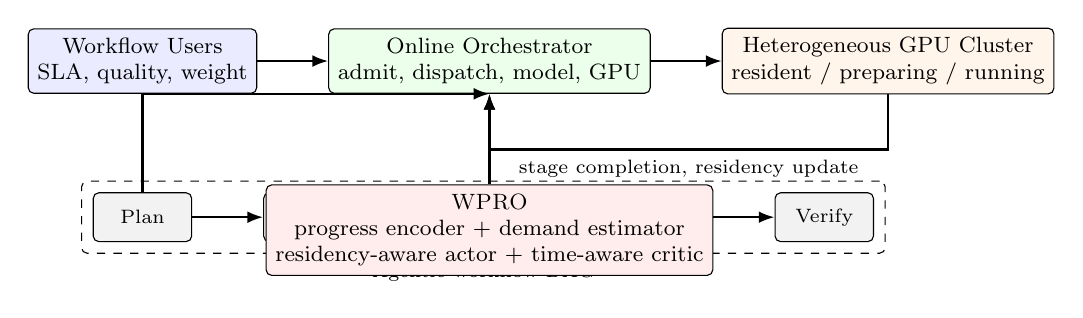
\begin{tikzpicture}[
        node distance=0.62cm and 0.9cm,
        box/.style={draw, rounded corners=2pt, align=center, minimum height=0.75cm, font=\footnotesize},
        stage/.style={draw, rounded corners=2pt, align=center, minimum height=0.62cm, minimum width=1.25cm, font=\scriptsize},
        arrow/.style={-{Latex[length=2mm]}, thick},
        dashedbox/.style={draw, dashed, rounded corners=2pt, inner sep=4pt}
    ]
    \node[box, fill=blue!8] (users) {Workflow Users\\SLA, quality, weight};
    \node[box, fill=green!8, right=of users, minimum width=2.1cm] (orch) {Online Orchestrator\\admit, dispatch, model, GPU};
    \node[box, fill=orange!8, right=of orch, minimum width=2.35cm] (cluster) {Heterogeneous GPU Cluster\\resident / preparing / running};
    \draw[arrow] (users) -- (orch);
    \draw[arrow] (orch) -- (cluster);
    \draw[arrow] (cluster.south) |- ++(0,-0.7) -| node[pos=0.25, below, font=\scriptsize] {stage completion, residency update} (orch.south);

    \node[stage, fill=gray!10, below=1.25cm of users] (p) {Plan};
    \node[stage, fill=gray!10, right=of p] (r) {Retrieve};
    \node[stage, fill=gray!10, right=of r] (rea) {Reason};
    \node[stage, fill=gray!10, right=of rea] (w) {Write};
    \node[stage, fill=gray!10, right=of w] (v) {Verify};
    \draw[arrow] (p) -- (r);
    \draw[arrow] (r) -- (rea);
    \draw[arrow] (rea) -- (w);
    \draw[arrow] (w) -- (v);
    \node[dashedbox, fit=(p)(r)(rea)(w)(v), label={[font=\scriptsize]below:Agentic workflow DAG}] {};

    \node[box, fill=red!7, below=1.15cm of orch, minimum width=3.8cm] (wpro) {\WPRO\\progress encoder + demand estimator\\residency-aware actor + time-aware critic};
    \draw[arrow] (p.north) |- (orch.south);
    \draw[arrow] (wpro.north) -- (orch.south);
    \end{tikzpicture}
    \caption{System overview and design intuition. Agentic workflows dynamically release stages. \WPRO\ observes both workflow progress and GPU model residency to make event-driven orchestration decisions.}
    \label{fig:system_design}
\end{figure*}

\subsection{Agentic Workflow Model}

Workflow requests arrive online. Let workflow \(j\in\calJ\) be represented by a directed acyclic graph \(G_j=(\calV_j,\calE_j)\), where each node \(i\in\calV_j\) is a stage and each edge \((i,i')\in\calE_j\) denotes a precedence constraint. A stage has semantic type \(q_{ji}\), execution class \(c_{ji}\in\{\textsf{llm},\textsf{tool},\textsf{communication}\}\), input tokens \(N^{\mathrm{in}}_{ji}\), expected output tokens \(N^{\mathrm{out}}_{ji}\), output size \(s_{ji}\), and model capability requirement. Workflow \(j\) arrives at \(a_j\), has deadline \(D_j\), and carries service-class weight \(w_j\).

At time \(t\), a stage is dependency-ready if all predecessors have completed and all required communication delay has elapsed. We denote the ready LLM stages by
\begin{equation}
\calR(t)=\{(j,i): c_{ji}=\textsf{llm},~i\notin C_j(t),~\mathrm{Pred}_j(i)\subseteq C_j(t),~r_{ji}\le t\},
\end{equation}
where \(C_j(t)\) is the set of completed stages and \(r_{ji}\) is the stage release time. Tool stages do not enter the GPU ready queue. Once their predecessors complete, they are automatically started and later generate completion events.

\subsection{Model Residency and Stage Latency}

Each GPU \(g\) has a resident model \(\rho_g(t)\), a target model under preparation \(\tilde{\rho}_g(t)\), and a running stage if the GPU is busy. The preparation latency for serving stage \((j,i)\) by model \(m\) on GPU \(g\) is
\begin{equation}
L^{\mathrm{prep}}_{g,m}(t)=
\begin{cases}
0, & \rho_g(t)=m,\\
L^{\mathrm{adapter}}_{g,m}, & m \text{ is adapter-compatible with } \rho_g(t),\\
L^{\mathrm{load}}_{g,m}, & \text{otherwise}.
\end{cases}
\end{equation}
The expected execution latency is token-aware:
\begin{equation}
\bar L^{\mathrm{exec}}_{ji,m,g} =
\alpha_{m,g}N^{\mathrm{in}}_{ji}+\beta_{m,g}N^{\mathrm{out}}_{ji}
\chi_{q_{ji},m,g}.
\end{equation}
The actual execution latency is sampled only when the dispatch is committed:
\begin{equation}
L^{\mathrm{exec}}_{ji,m,g}=\bar L^{\mathrm{exec}}_{ji,m,g}\xi_{ji,m,g},
\end{equation}
where \(\xi_{ji,m,g}\) captures runtime perturbation. This separation prevents policy scoring from consuming random numbers and keeps baseline evaluation fair.

If successor \(i'\) is placed after predecessor \(i\), its release time includes communication:
\begin{equation}
L^{\mathrm{com}}_{ji,i',g,g'}=\ell_{g,g'} + \frac{s_{ji}}{B_{g,g'}},
\end{equation}
where \(\ell_{g,g'}\) is network latency and \(B_{g,g'}\) is bandwidth.

\subsection{Online Decision and Objective}

At orchestration event \(n\), the system state is \(S_n\) and the event time is \(t_n\). The action contains admission decisions and assignments for idle GPUs:
\begin{equation}
A_n=\{x_j\}_{j\in\calJ_n^{\mathrm{arr}}}\cup \{a_{n,g}:g\in\calI_n\},
\end{equation}
where \(x_j\in\{0,1\}\) admits or rejects an arriving workflow, \(\calI_n\) is the idle GPU set, and
\begin{equation}
a_{n,g}\in \{(j,i,m,g):(j,i)\in\calR(t_n),~m\in\calM_{ji},~b_m\le B_g\}\cup\{\textsf{WAIT}_g\}.
\end{equation}
Assignments must not dispatch the same stage twice at the same event.

The platform maximizes weighted SLA-compliant completed value:
\begin{equation}
\max_{\pi}~\mathbb{E}_{\pi}\left[\sum_{j\in\calJ} w_j
\ind\{T_j-a_j\le D_j,~j\text{ completed}\}\right],
\label{eq:objective}
\end{equation}
subject to precedence, capability, GPU-memory, admission, and timing constraints. We also report the weighted goodput rate
\begin{equation}
G_{\mathrm{w}}=\frac{1}{T_{\mathrm{episode}}}
\sum_j w_j\ind\{T_j-a_j\le D_j\}.
\end{equation}

\subsection{Problem Hardness and Bellman Coupling}

\textbf{Theorem 1.} The offline version of problem \eqref{eq:objective} is NP-hard.

\textit{Proof sketch.} Consider a restricted instance with one event, independent one-stage workflows, one GPU, no communication, no tool stages, and known execution time. Each workflow has value \(w_j\), processing time \(p_j\), and a common deadline equal to GPU capacity \(C\). Selecting workflows to complete before the deadline is equivalent to selecting items with weights \(p_j\) and values \(w_j\) under capacity \(C\), which contains the 0--1 knapsack problem. Therefore, the restricted problem is NP-hard, and the general orchestration problem is NP-hard. \(\square\)

More importantly, online orchestration has Bellman coupling. The next state satisfies
\begin{equation}
S_{n+1}=F(S_n,A_n,\omega_n),
\end{equation}
where \(A_n\) changes both \(C_j(t)\) and \(\rho_g(t)\). Hence the value recursion is
\begin{equation}
V^{\pi}(S_n)=\mathbb{E}_{\pi}\left[R_n + e^{-\beta\Delta t_n}V^{\pi}(S_{n+1})\mid S_n\right].
\end{equation}
A greedy scheduler that maximizes only \(R_n\) ignores the impact of \(A_n\) on future ready-stage release and model preparation cost.

\section{The \WPRO\ Framework}

\subsection{SMDP Formulation}

We model online orchestration as an event-driven SMDP. Events are workflow arrivals, tool-stage completions, model-preparation completions, LLM-stage completions, deadline drops, and idle-GPU decisions. The transition interval \(\Delta t_n=t_{n+1}-t_n\) is nonuniform, so \WPRO\ uses a time-aware discount \(\gamma_n=e^{-\beta\Delta t_n}\). The reward contains terminal weighted value, resource costs, and optional potential-based shaping:
\begin{equation}
R_n=R_n^{\mathrm{terminal}}-\lambda_{\mathrm{prep}}C_n^{\mathrm{prep}}
-\lambda_{\mathrm{drop}}C_n^{\mathrm{drop}}+
\ind_{\mathrm{shape}}\left(\gamma_n\Phi(S_{n+1})-\Phi(S_n)\right).
\end{equation}
The shaping potential is designed so that progress increases potential but pure waiting with shrinking slack does not:
\begin{equation}
\Phi(S)=\sum_{j\in\calJ^{\mathrm{act}}} w_j \alpha_j(S)
\mathrm{clip}\left(\frac{\mathrm{slack}_j(S)}{D_j},0,1\right),
\end{equation}
where
\begin{equation}
\alpha_j(S)=\frac{1}{2}\rho_j^{\mathrm{node}}(S)+
\frac{1}{2}\rho_j^{\mathrm{cp}}(S).
\end{equation}
Here \(\rho_j^{\mathrm{node}}\) is the completed-node ratio and \(\rho_j^{\mathrm{cp}}\) is the completed critical-path ratio.

\subsection{Workflow-Progress Encoder}

For each active workflow \(j\), \WPRO\ encodes not only the currently ready node but also future demand implied by unfinished DAG structure. The workflow feature vector includes completed-stage ratio, ready-stage ratio, remaining critical path, slack ratio, service-class weight, mean ready waiting time, successor-stage type histogram, and remaining-stage type histogram. A permutation-invariant pooling operator aggregates active workflows:
\begin{equation}
h_{\mathrm{wf}}=\mathrm{Pool}\{f_{\theta}^{\mathrm{wf}}(W_j):j\in\calJ^{\mathrm{act}}\}.
\end{equation}
The GPU set is encoded similarly:
\begin{equation}
h_{\mathrm{gpu}}=\mathrm{Pool}\{f_{\theta}^{\mathrm{gpu}}(g,\rho_g,\tilde{\rho}_g):g\in\calG\}.
\end{equation}
The global state embedding is \(h_S=[h_{\mathrm{wf}},h_{\mathrm{gpu}},h_{\mathrm{sys}}]\).

\subsection{DAG-Induced Future Model-Demand Estimator}

For each model \(m\), \WPRO\ estimates the near-future demand within horizon \(H\):
\begin{equation}
\hat d_m(H\mid S_n)=f_{\psi}^{\mathrm{dem}}(h_S,m).
\end{equation}
The auxiliary label is the DAG-induced near-future demand \(d_m^{\mathrm{DAG}}(H\mid S_n)\), computed from unfinished workflow DAGs, dependency release estimates, slack, and model feasibility. We deliberately do not call it true future rollout demand, because future arrivals and stochastic branch outcomes remain unknown. The auxiliary objective is
\begin{equation}
\mathcal{L}_{\mathrm{dem}}(\psi)=
\sum_{m\in\calM}
\left(\hat d_m(H\mid S_n)-d_m^{\mathrm{DAG}}(H\mid S_n)\right)^2.
\end{equation}
This head gives the actor an explicit representation of future model pressure induced by active workflows.

\subsection{Residency-Aware Action Scoring}

For each candidate assignment \(a=(j,i,m,g)\), \WPRO\ builds action-specific features:
\begin{equation}
\phia(S,a)=
[h_S,h_j,h_i,h_m,h_g,h_{\mathrm{cross}}],
\end{equation}
where \(h_{\mathrm{cross}}\) includes slack, remaining critical path, preparation time, expected execution time, resident hit, adapter compatibility, predicted target-model demand \(\hat d_m(H)\), and predicted demand for the currently resident model \(\hat d_{\rho_g}(H)\). A structural residency term is
\begin{equation}
\Delta\Psi_{j,i,m,g}=
\hat d_m(H)-\hat d_{\rho_g}(H)-\lambda L_{g,m}^{\mathrm{prep}}.
\end{equation}
The actor logit is
\begin{equation}
\ell_{\theta}(S,a)=\theta^\top\phia(S,a)+\eta\Delta\Psi_{j,i,m,g}.
\label{eq:logit}
\end{equation}
Unlike a state-only actor, \eqref{eq:logit} can learn relative preferences among candidate actions within the same decision event.

\subsection{Event-Aware Autoregressive Matching Decoder}

Enumerating all stage--model--GPU dispatch matrices is infeasible. \WPRO\ processes idle GPUs in a fixed order and updates the feasible set after each selection:
\begin{equation}
\pi_{\theta}(A_n\mid S_n)=
\prod_{g\in\calI_n}
\pi_{\theta}(a_{n,g}\mid S_n,a_{n,<g}).
\end{equation}
The WAIT action lets \WPRO\ keep a GPU idle until the next exogenous event when immediate dispatch would destroy valuable residency.

\begin{algorithm}[t]
\caption{\WPRO\ Event-Driven Orchestration}
\label{alg:wpro}
\begin{algorithmic}[1]
\State Initialize actor \(\theta\), critic \(\phi\), demand estimator \(\psi\)
\For{episode \(=1,\ldots,E\)}
    \State Reset environment and event clock
    \While{episode not terminated}
        \State Observe \(S_n\), ready set \(\calR(t_n)\), idle GPUs \(\calI_n\)
        \State Encode workflow progress and GPU residency into \(h_S\)
        \State Estimate \(\hat d_m(H\mid S_n)\) for all \(m\in\calM\)
        \State \(A_n\gets\emptyset\), used stages \(\gets\emptyset\)
        \For{idle GPU \(g\in\calI_n\)}
            \State Build feasible candidates \(\calA_g(S_n)\cup\{\textsf{WAIT}_g\}\)
            \State Compute logits by \eqref{eq:logit}
            \State Sample or select \(a_{n,g}\sim\pi_\theta(\cdot\mid S_n,a_{n,<g})\)
            \State Remove dispatched stage from later candidate sets
        \EndFor
        \State Execute assignments, sample committed execution time once
        \State Store \((S_n,A_n,R_n,\Delta t_n,S_{n+1})\)
    \EndWhile
    \State Compute time-aware GAE with frozen critic values
    \State Update actor, critic, and demand estimator
\EndFor
\end{algorithmic}
\end{algorithm}

\subsection{Time-Aware Critic and Policy Update}

The critic estimates \(V_{\phi}(S_n)\). For transition \(n\), the TD residual is
\begin{equation}
\delta_n=R_n+e^{-\beta\Delta t_n}V_{\phi}(S_{n+1})-V_{\phi}(S_n).
\end{equation}
The time-aware GAE is
\begin{equation}
\hat A_n=\sum_{k\ge 0}
\left(\prod_{\ell=0}^{k-1} e^{-\beta\Delta t_{n+\ell}}\lambda_{\mathrm{GAE}}\right)
\delta_{n+k}.
\end{equation}
Actor gradients use the correct action-feature softmax gradient:
\begin{equation}
\nabla_{\theta}\log\pi_{\theta}(a\mid S)=
\phia(S,a)-\sum_{a'\in\calA(S)}\pi_{\theta}(a'\mid S)\phia(S,a').
\end{equation}
The critic is updated to fit \(\hat G_n=\hat A_n+V_{\phi}(S_n)\), while the demand estimator is trained with \(\mathcal{L}_{\mathrm{dem}}\).

\section{Experimental Methodology}

\subsection{Simulator and Workloads}

We implement an event-driven simulator for agentic AIaaS orchestration. Workflows contain LLM stages, tool stages, and communication stages. LLM stages require model/GPU selection; tool stages run outside the GPU queue and generate completion events; communication delay affects successor release time. LLM execution time is token-dependent and stochastic only at committed execution. Model residency is represented by a GPU state machine with resident, preparing, and running states.

For trace-driven experiments, public LLM-serving traces such as BurstGPT \cite{wang2024burstgpt} are converted into workflow arrivals with token lengths and workload intensity. To avoid leakage, traces are split chronologically into training, validation, and test segments with guard intervals around split boundaries. The policy is trained on the training split, checkpointed by validation performance, and evaluated on held-out test windows.

\subsection{Baselines}

Table~\ref{tab:baselines} summarizes the baseline adaptation. All methods run in the same simulator and differ only in orchestration policy.

\begin{table*}[t]
\centering
\caption{Baseline adaptation under the unified evaluation framework.}
\label{tab:baselines}
\begin{tabular}{lllll}
\toprule
Method & Admission & Stage priority & Model/GPU selection & Notes \\
\midrule
FCFS & shared & earliest admitted workflow & earliest local finish & classical queue baseline \\
EDF & shared & earliest deadline & earliest local finish & deadline-aware online baseline \\
SRPT & shared & least remaining critical path & earliest local finish & short-workflow baseline \\
Utility-Greedy & shared & utility/slack score & myopic prep/exec score & current ready queue only \\
Lyapunov & shared & drift-plus-penalty & greedy matching & queueing-control baseline \\
DAG-Oracle Greedy & shared & oracle DAG demand & residency-aware greedy & strong oracle heuristic \\
Vanilla A2C & shared & learned & learned & same A2C without WPRO modules \\
PPO & shared & learned & learned & generic RL baseline \\
vLLM/Orca/Sarathi-inspired & shared & runtime-inspired queueing & runtime-inspired batching & adaptation, not full system reproduction \\
\WPRO & shared & learned progress-aware & residency-aware actor & proposed method \\
\bottomrule
\end{tabular}
\end{table*}

\subsection{Metrics and Statistical Protocol}

We report weighted completed value \(V_{\mathrm{w}}\), weighted goodput rate \(G_{\mathrm{w}}\), admission ratio \(R_{\mathrm{adm}}\), on-time completion ratio \(R_{\mathrm{on}}\), conditional SLA success ratio, P95 latency, residency hit ratio, model full-load count, model preparation time, communication overhead, queue waiting time, demand-prediction error, and decision overhead. For final experiments, we use five independent RL training seeds, at least twenty paired held-out test windows per configuration, validation checkpoint selection, bootstrap 95\% confidence intervals, and Wilcoxon signed-rank tests against the strongest online baseline.

\section{Evaluation}

\subsection{Overall Performance}

Fig.~\ref{fig:overall} compares normalized utility, admission ratio, and on-time completion ratio. The important trend is not simply that \WPRO\ admits the most workflows. In fact, aggressive admission can reduce SLA success when load is high. \WPRO\ improves weighted utility by admitting and dispatching workflows whose downstream DAG structure and residency implications make them more likely to complete before deadline.

\begin{figure*}[t]
    \centering
    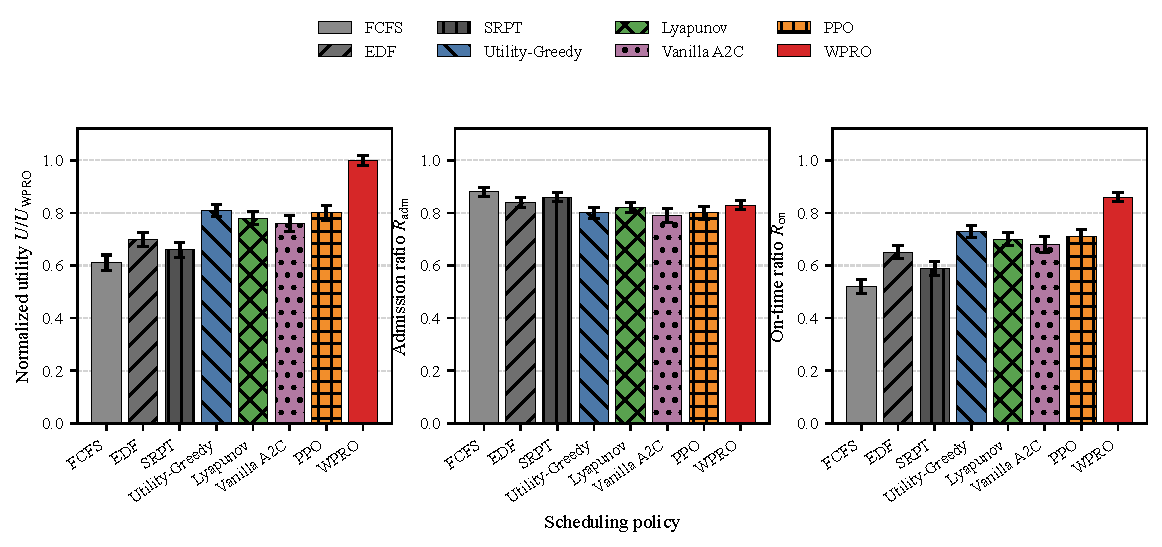
\includegraphics[width=0.95\linewidth]{../paper_artifacts/figures/fig1_overall_performance.pdf}
    \caption{Overall performance across representative policies. Error bars denote 95\% confidence intervals over paired test windows.}
    \label{fig:overall}
\end{figure*}

\subsection{Scalability with Arrival Rate}

Fig.~\ref{fig:scalability} shows performance as arrival rate \(\lambda\) increases. Under light load, most online policies can serve requests before deadlines. Under heavier load, residency mistakes become more expensive because cold loads block GPUs and delay many downstream stages. \WPRO\ maintains higher goodput and on-time completion by using future demand and WAIT decisions.

\begin{figure*}[t]
    \centering
    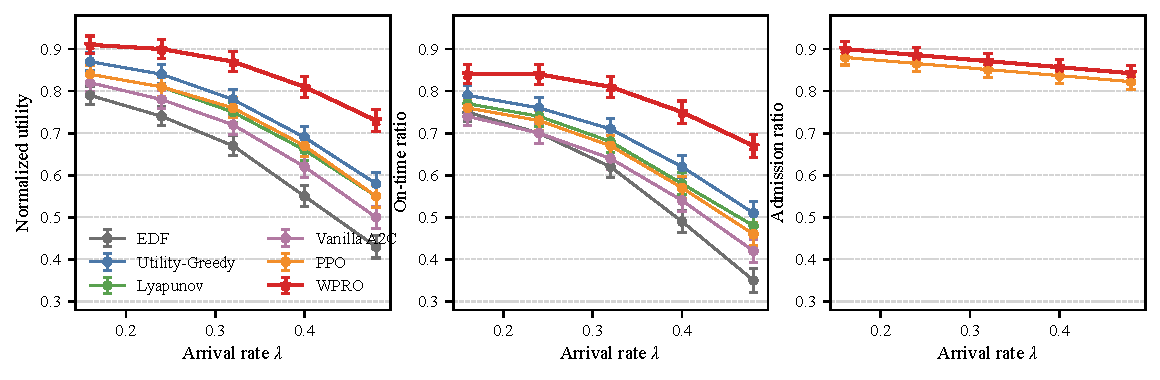
\includegraphics[width=0.95\linewidth]{../paper_artifacts/figures/fig2_scalability_vs_arrival_rate.pdf}
    \caption{Scalability with workload arrival rate. \WPRO\ is expected to show larger gains under heavy load, where future model demand and residency decisions matter more.}
    \label{fig:scalability}
\end{figure*}

\subsection{Robustness Across Workload Settings}

Fig.~\ref{fig:robustness} compares \WPRO\ with the strongest baseline in each workload setting. Points above the \(y=x\) line indicate that \WPRO\ improves utility. This view is useful because the strongest baseline may change across settings: EDF can be strong under tight deadlines, while Utility-Greedy can be strong under moderate load.

\begin{figure}[t]
    \centering
    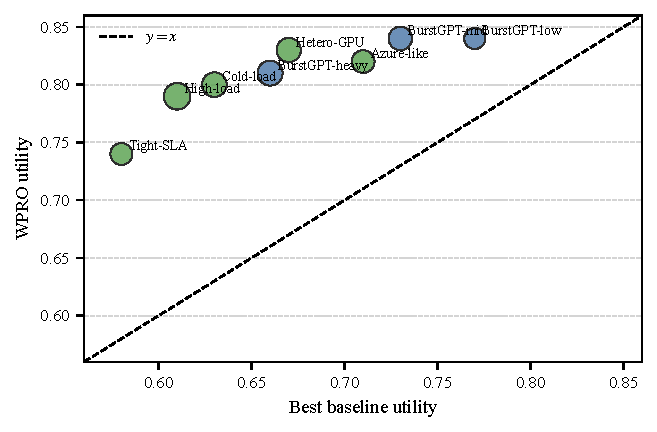
\includegraphics[width=\linewidth]{../paper_artifacts/figures/fig3_multi_environment_improvement.pdf}
    \caption{Multi-environment robustness. Each point is a workload setting; marker size denotes number of workflows.}
    \label{fig:robustness}
\end{figure}

\subsection{Deadline Tightness and Workflow Complexity}

Fig.~\ref{fig:surface} studies the interaction between deadline tightness and DAG complexity. Larger DAGs release more future stages and create more opportunities for residency-aware scheduling. Tighter deadlines reduce slack and make cold-load mistakes more damaging.

\begin{figure}[t]
    \centering
    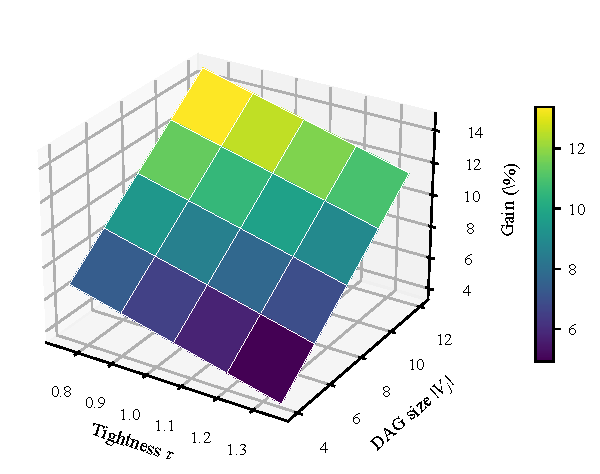
\includegraphics[width=\linewidth]{../paper_artifacts/figures/fig4_deadline_complexity_surface.pdf}
    \caption{Utility gain of \WPRO\ over the strongest online baseline as deadline tightness and DAG size vary.}
    \label{fig:surface}
\end{figure}

\subsection{Latency Breakdown}

Fig.~\ref{fig:breakdown} decomposes workflow latency into queue waiting, model preparation, communication, and token execution. \WPRO\ mainly reduces queue waiting and model preparation. This is consistent with the design: the algorithm does not claim to reduce unavoidable token execution time; instead, it improves orchestration decisions that determine when stages wait and when GPUs cold-load models.

\begin{figure}[t]
    \centering
    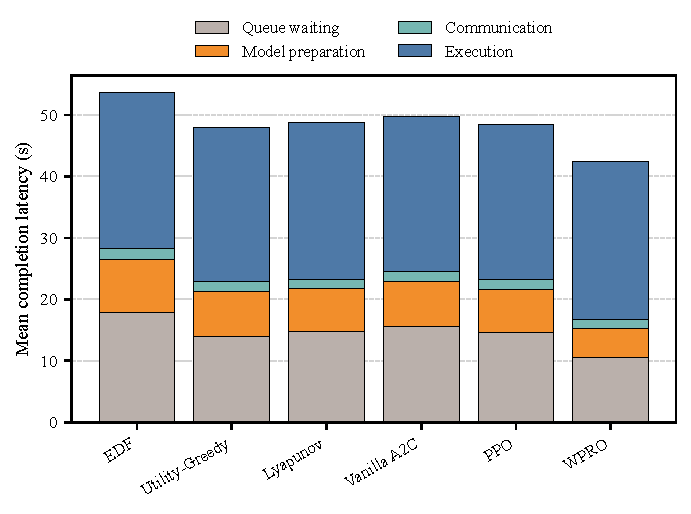
\includegraphics[width=\linewidth]{../paper_artifacts/figures/fig5_latency_breakdown.pdf}
    \caption{Latency breakdown. \WPRO\ reduces queue waiting and preparation overhead through residency-aware orchestration.}
    \label{fig:breakdown}
\end{figure}

\subsection{Mechanism Analysis}

Fig.~\ref{fig:mechanism} examines two mechanisms. The left panel compares predicted demand \(\hat d_m(H)\) with DAG-induced labels \(d_m^{\mathrm{DAG}}(H)\). The right panel shows residency hit ratio under increasing arrival rate. Better near-future demand estimation helps the actor preserve useful resident models and avoid unnecessary full loads.

\begin{figure*}[t]
    \centering
    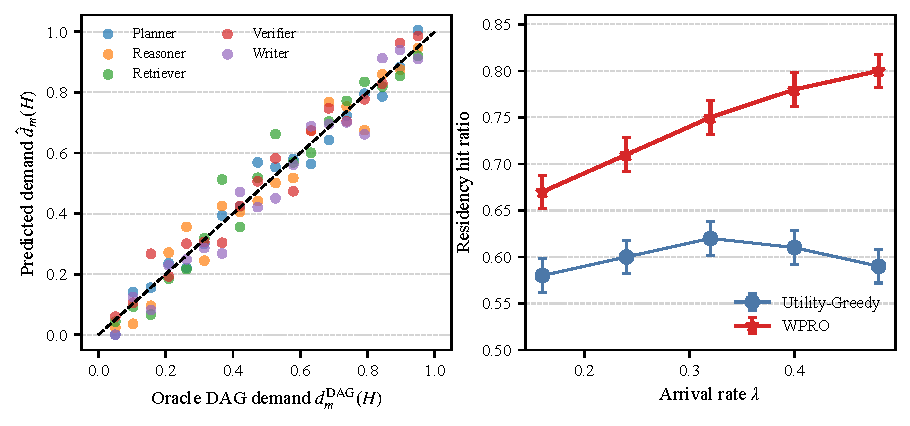
\includegraphics[width=0.78\linewidth]{../paper_artifacts/figures/fig6_demand_prediction_and_residency.pdf}
    \caption{Mechanism analysis: demand-estimation quality and residency hit ratio.}
    \label{fig:mechanism}
\end{figure*}

\subsection{Ablation Study}

Fig.~\ref{fig:ablation} removes key modules from \WPRO. Removing the demand estimator weakens anticipation of future model pressure; removing residency features weakens model-retention decisions; removing workflow progress reduces awareness of unfinished DAG structure; removing WAIT prevents the policy from preserving residency for imminent high-value stages.

\begin{figure*}[t]
    \centering
    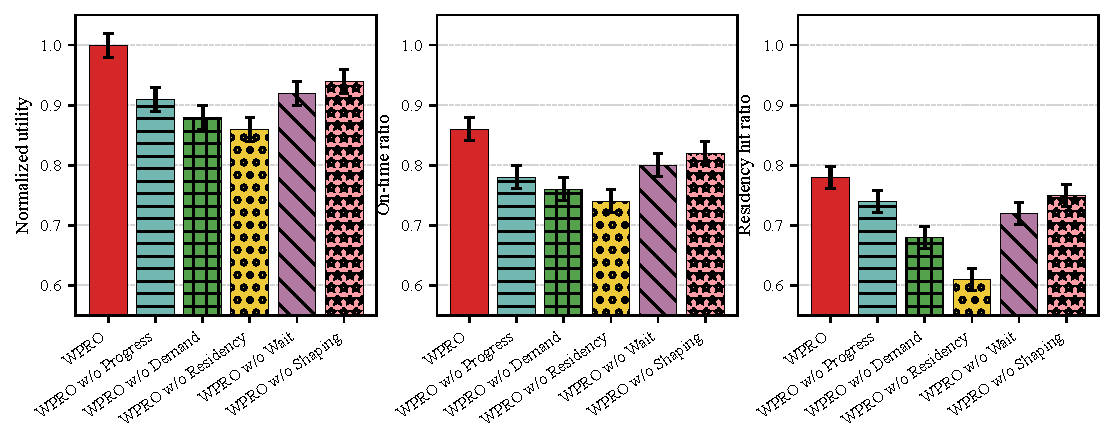
\includegraphics[width=0.95\linewidth]{../paper_artifacts/figures/fig7_ablation_study.pdf}
    \caption{Ablation study over WPRO modules.}
    \label{fig:ablation}
\end{figure*}

\subsection{Scheduling Behavior and Overhead}

Fig.~\ref{fig:overhead} visualizes a representative scheduling timeline and policy overhead. The timeline highlights resident hits and cold loads. The overhead plot shows that the autoregressive decoder scales with the number of candidate actions without enumerating full dispatch matrices.

\begin{figure*}[t]
    \centering
    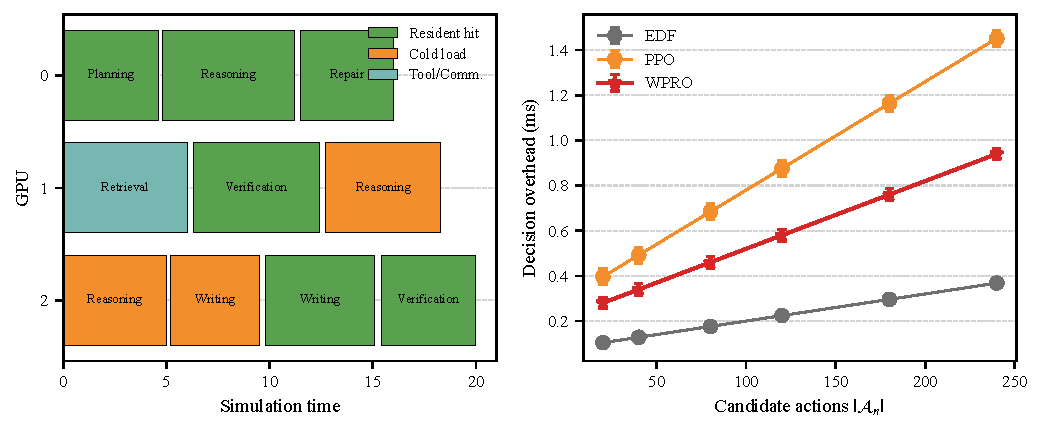
\includegraphics[width=0.85\linewidth]{../paper_artifacts/figures/fig8_schedule_timeline_and_overhead.pdf}
    \caption{Scheduling behavior and decision overhead.}
    \label{fig:overhead}
\end{figure*}

\section{Discussion}

\subsection{Why Not Claim Full vLLM/Orca/Sarathi Comparison?}

Systems such as vLLM, Orca, and Sarathi-Serve optimize low-level LLM inference execution. They are not workflow orchestrators that jointly decide admission, stage dispatch, model selection, and GPU assignment for agentic DAGs. Therefore, a fair comparison should either integrate \WPRO\ on top of these runtimes or adapt their scheduling principles within the same simulator. This paper follows the latter approach for baseline design and avoids claiming full-system reproduction.

\subsection{Limitations}

The current demand estimator uses a DAG-induced auxiliary label rather than the actual future rollout. This is appropriate when active workflow DAGs are visible, but it does not capture unobserved future arrivals or conditional branches unless those are modeled in the workload generator. A future version can extend the simulator with probabilistic repair branches, retry behavior, and unknown tool outcomes. In addition, strict optimality gaps require CP-SAT/MILP or complete enumeration on small instances; bounded lookahead should only be described as a reference.

\section{Conclusion}

We presented \WPRO, a workflow-progress and residency-aware orchestration framework for online agentic LLM services. The central insight is that completing a workflow stage changes future executable stages, while selecting a model changes GPU residency and future preparation latency. \WPRO\ captures this coupling through structured actor--critic learning with workflow-progress encoding, DAG-induced demand estimation, residency-aware action scoring, autoregressive matching, WAIT decisions, and time-aware value estimation. The proposed trace-driven evaluation framework provides a reproducible path toward INFOCOM-style evidence: isolated data splits, paired workload evaluation, confidence intervals, strong online baselines, RL baselines, and mechanism-level ablations.

\bibliographystyle{IEEEtran}
\bibliography{references}

\end{document}
